\section{Auswertung}

\subsection{Versuchsabschnitt A}

\subsubsection*{Messdaten}

Zunächst müssen wir die in der Durchführung gesammelten Daten weiter verarbeiten.
Unser LabVIEW-Skript speichert $U_T$, $f$, $U_X$ und $U_Y$ - jeweils in einer Spalte.
Dabei bezeichnet $U_T$ die Spannung am Pt-1000-Widerstandsthermometer, $f$ die eingestellte Frequenz am Frequenzgenerator sowie $U_X$ beziehungsweise $U_Y$ die beiden Ausgangskanäle des Verstärkers.

Wir mitteln die je 20 Messdaten für $U_X$ und $U_Y$, welche wir für jede der Frequenzen aufgenommen haben.
Für die Temperatur können weitaus mehr Messpunkte gemittelt werden, sodass am Ende 11 Werte insgesamt entstehen.
Zu den Mittelwerten berechnen wir ebenso den Mittleren Fehler des Mittelwerts.

Aus der Frequenz $f$ des Frequenzgenerators bestimmen wir die Frequenz $\omega$ der Schwingung mit den Informationen von Gleichung \ref{eq:PeriodischeKraft} nach
\begin{align}
    \omega &= 2 \pi (2f) = 4 \pi f.
\end{align}

Für die Spannung $U_T$ am Pt-1000-Widerstandsthermometer gilt die Formel
\begin{align}
    T &= 259.2684 \left ( U_T - 1.000325 \right )
\end{align}

zur Berechnung der Temperatur.

Um die zur Verfügung stehenden Messdaten $U_X$ und $U_Y$ weiter zu untersuchen, nutzen wir die Beziehung
\begin{align}
    U_X &= A \sin \Phi
    \intertext{und}
    U_Y &= A \cos \Phi
\end{align}

aus, sodass sich als weitere Größen Amplitude
\begin{align}
    A &= \sqrt{U_X^2 + U_Y^2}
    \intertext{und Phase}
    \Phi &= \arctan \frac{U_Y}{U_X}
\end{align}

ergeben.

\subsubsection*{Ordinary-Least-Squares Fit}

Wie im vorherigen Abschnitt beschrieben, sind nun also Messdaten für die Gleichungen \ref{eq:Phase}, \ref{eq:Lorentzkurve}, \ref{eq:PhaseSin} sowie \ref{eq:PhaseCos} vorhanden und können mithilfe eines Ordinary-Least-Squares (OLS) Fit angepasst werden.

Dafür nutzen wir das für Python verfügbare \texttt{scipy.odr} Modul.
Die freien Argumente der Gleichungen - beispielsweise die Amplitude $f_0$, die Eigenfrequenz $\omega_0$ oder die Dämpfung $\gamma$ - stellen die Parameter des Fits.
Aus dem Fit ergeben sich also Werte für diese Parameter.
Die entsprechenden Fehler beziehungsweise fortgepflanzten Messunsicherheiten ergeben sich aus der Wurzel der Diagonaleinträge der Kovarianzmatrix.
Den Bereich der Fits wählen wir nach Augenmaß so, dass einerseits keine offensichtlichen Messfehler beitragen, und andererseits, dass das Modell überhaupt theoretisch Gültigkeit in diesem Bereich besitzt.
(Beispielsweise beschreibt die Lorentzkurve den Amplitudenverlauf nur in unmittelbarer Nähe der Resonanzfrequenz.)

Für den Fit und Plot von $A$ fügen wir außerdem die normierten Abweichungen (residuals) nach $\frac{A_i - \zeta_{Fit}(\omega_i)}{\delta_i}$ in die Abbildung ein.
Dabei beschreibt $A_i$ den Messwert, $\zeta_{Fit}(\omega_i)$ den Wert der resultierten Fitfunktion an der gleichen Stelle und $\delta_i$ die Messunsicherheit.

Um die Qualität des Fits zu burteilen bestimmen wir die Anzahl der Freiheitsgrade des Fits dof (degrees of freedom), die Fiteigenschaften $\chi^2$ und $\chi^2_{red}$ sowie schließlich die Fitwahrscheinlichkeit prob.
Dabei beschreibt prob die Wahrscheinlichkeit, dass unter Zugrundelegung des verwendeten Modells, Daten mit dem gemessenen oder einem höheren $\chi^2$ zu erhalten.
Die Wahrscheinlichkeitsdichtefunktion ist im Modul \texttt{scipy.stats} enthalten.

\subsubsection*{Resonanzfrequenz $\omega_R$ und Güte $Q$}

Aus den per Fit berechneten Parametern lässt sich nun die Resonanzfrequenz $\omega_R$ nach Gleichung \ref{eq:Resonanzfrequenz} bestimmen.
Gleiches gilt für die Güte $Q$ nach Gleichung \ref{eq:Guete}.

Zusätzlich bestimmen wir die volle Breite FW (full width) der Lorentzkurve auf der Höhe des $\frac{1}{\sqrt{2}}$-fachen Maximums.

\subsubsection*{Ergebnisse}

Die Ergebnisse der oben besprochenen Auswertung sind in Tabelle \ref{tab:FitErgebnisse} aufgetragen.
Ausgewählte Plots sind in Abbildung \ref{fig:RaumtempKomplett} und \ref{fig:FehlersucheMode3} dargestellt.

\minipage{\linewidth}
    \begin{center}
        \captionsetup{type=table}
        \begin{adjustbox}{max width=\linewidth, keepaspectratio}
            \begin{tabular}{lllll}
            \toprule
            Daten & Eigenschaften & 1. Mode ($\nu_0$) & 2. Mode ($\nu_1$) & 3. Mode ($\nu_2$) \\
            \midrule
            A & $\omega_0$ [$s^{-1}$] & (2.004632$\pm$0.000047)$\;\cdot\; 10^{3}$ & (1.248063$\pm$0.000011)$\;\cdot\; 10^{4}$ & (3.532$\pm$0.020)$\;\cdot\; 10^{4}$ \\
            ~ & $\gamma$ [$s^{-1}$] & (3.394$\pm$0.011)$\;\cdot\; 10^{1}$ & (5.520$\pm$0.026)$\;\cdot\; 10^{1}$ & (8.25$\pm$0.37)$\;\cdot\; 10^{2}$ \\
            ~ & dof & 130 & 130 & 130 \\
            ~ & $\chi^2$ & 140 & 230 & 280 \\
            ~ & $\chi_{red}^2$ & 1.1 & 1.7 & 2.1 \\
            ~ & prob & 0.23 & 0.00000044 & 0.0 \\
            ~ & $\omega_R$ [$s^{-1}$] & (2.004488$\pm$0.000047)$\;\cdot\; 10^{3}$ & (1.248057$\pm$0.000011)$\;\cdot\; 10^{4}$ & (3.532$\pm$0.020)$\;\cdot\; 10^{4}$ \\
            ~ & Q & (5.906$\pm$0.019)$\;\cdot\; 10^{1}$ & (2.261$\pm$0.011)$\;\cdot\; 10^{2}$ & (4.28$\pm$0.19)$\;\cdot\; 10^{1}$ \\
            $\Phi$ & $\omega_0$ [$s^{-1}$] & (2.005142$\pm$0.000039)$\;\cdot\; 10^{3}$ & (1.2487628$\pm$0.0000067)$\;\cdot\; 10^{4}$ & (2$\pm$40)$\;\cdot\; 10^{5}$ \\
            ~ & $\gamma$ [$s^{-1}$] & (3.4608$\pm$0.0093)$\;\cdot\; 10^{1}$ & (6.854$\pm$0.028)$\;\cdot\; 10^{1}$ & (9$\pm$430)$\;\cdot\; 10^{5}$ \\
            ~ & dof & 130 & 130 & 130 \\
            ~ & $\chi^2$ & 390 & 2600 & 370 \\
            ~ & $\chi_{red}^2$ & 3.0 & 20 & 2.8 \\
            ~ & prob & 0.0 & 0.0 & 0.0 \\
            ~ & $\omega_R$ [$s^{-1}$] & (2.004993$\pm$0.000039)$\;\cdot\; 10^{3}$ & (1.2487533$\pm$0.0000067)$\;\cdot\; 10^{4}$ & (6$\pm$320)$\;\cdot\; 10^{5}$ \\
            ~ & Q & (5.794$\pm$0.016)$\;\cdot\; 10^{1}$ & (1.8220$\pm$0.0074)$\;\cdot\; 10^{2}$ & (2$\pm$99)$\;\cdot\; 10^{-1}$ \\
            X & $\omega_0$ [$s^{-1}$] & (2.004861$\pm$0.000048)$\;\cdot\; 10^{3}$ & (1.2486315$\pm$0.0000076)$\;\cdot\; 10^{4}$ & (3.5215$\pm$0.0035)$\;\cdot\; 10^{4}$ \\
            ~ & $\gamma$ [$s^{-1}$] & (3.394$\pm$0.011)$\;\cdot\; 10^{1}$ & (5.790$\pm$0.031)$\;\cdot\; 10^{1}$ & (3.07$\pm$0.16)$\;\cdot\; 10^{2}$ \\
            ~ & dof & 130 & 130 & 130 \\
            ~ & $\chi^2$ & 270 & 4500 & 220 \\
            ~ & $\chi_{red}^2$ & 2.1 & 35 & 1.7 \\
            ~ & prob & 0.0 & 0.0 & 0.0000010 \\
            ~ & $\omega_R$ [$s^{-1}$] & (2.004718$\pm$0.000048)$\;\cdot\; 10^{3}$ & (1.2486248$\pm$0.0000076)$\;\cdot\; 10^{4}$ & (3.5214$\pm$0.0035)$\;\cdot\; 10^{4}$ \\
            ~ & Q & (5.908$\pm$0.019)$\;\cdot\; 10^{1}$ & (2.156$\pm$0.011)$\;\cdot\; 10^{2}$ & (1.146$\pm$0.061)$\;\cdot\; 10^{2}$ \\
            Y & $\omega_0$ [$s^{-1}$] & (2.004973$\pm$0.000037)$\;\cdot\; 10^{3}$ & (1.2485031$\pm$0.0000081)$\;\cdot\; 10^{4}$ & (3.58$\pm$0.25)$\;\cdot\; 10^{4}$ \\
            ~ & $\gamma$ [$s^{-1}$] & (3.4444$\pm$0.0094)$\;\cdot\; 10^{1}$ & (6.302$\pm$0.024)$\;\cdot\; 10^{1}$ & (2.8$\pm$2.3)$\;\cdot\; 10^{3}$ \\
            ~ & dof & 130 & 130 & 130 \\
            ~ & $\chi^2$ & 330 & 1200 & 260 \\
            ~ & $\chi_{red}^2$ & 2.5 & 9.5 & 2.0 \\
            ~ & prob & 0.0 & 0.0 & 0.00000000032 \\
            ~ & $\omega_R$ [$s^{-1}$] & (2.004825$\pm$0.000037)$\;\cdot\; 10^{3}$ & (1.2484951$\pm$0.0000081)$\;\cdot\; 10^{4}$ & (3.58$\pm$0.25)$\;\cdot\; 10^{4}$ \\
            ~ & Q & (5.821$\pm$0.016)$\;\cdot\; 10^{1}$ & (1.9811$\pm$0.0075)$\;\cdot\; 10^{2}$ & (1.3$\pm$1.0)$\;\cdot\; 10^{1}$ \\
            \bottomrule
            \end{tabular}
        \end{adjustbox}
        \captionof{table}{Ergebnisse der Ordinary-Least-Squares Fits für die drei Schwingungsmoden $\nu_0$, $\nu_1$ und $\nu_2$ bei Raumtemperatur}
        \label{tab:FitErgebnisse}
    \end{center}
\endminipage

\minipage{\linewidth}
    \begin{center}
        \captionsetup{type=figure}
        \begin{adjustbox}{max width=0.45\linewidth, keepaspectratio}
            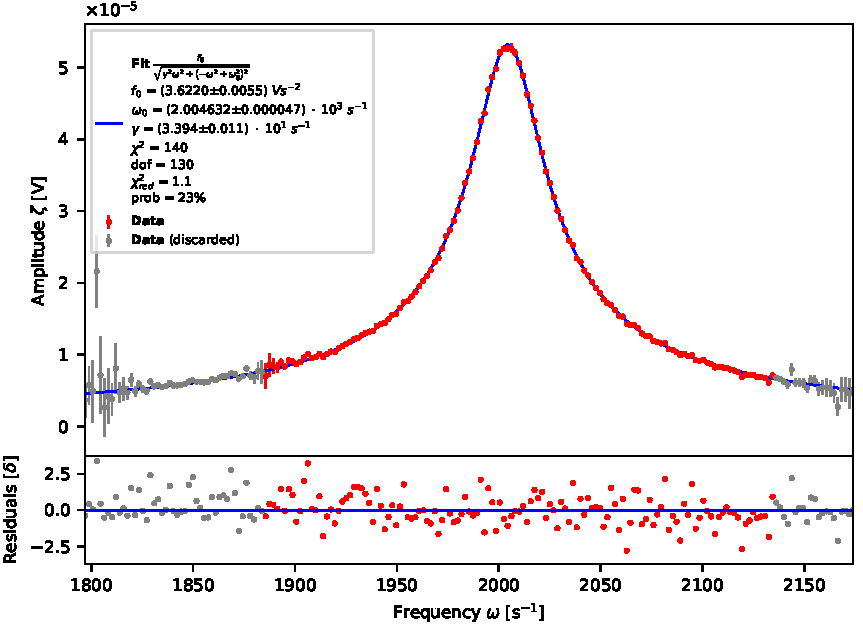
\includegraphics[]{pdf/A_0_0}
        \end{adjustbox}
        \begin{adjustbox}{max width=0.45\linewidth, keepaspectratio}
            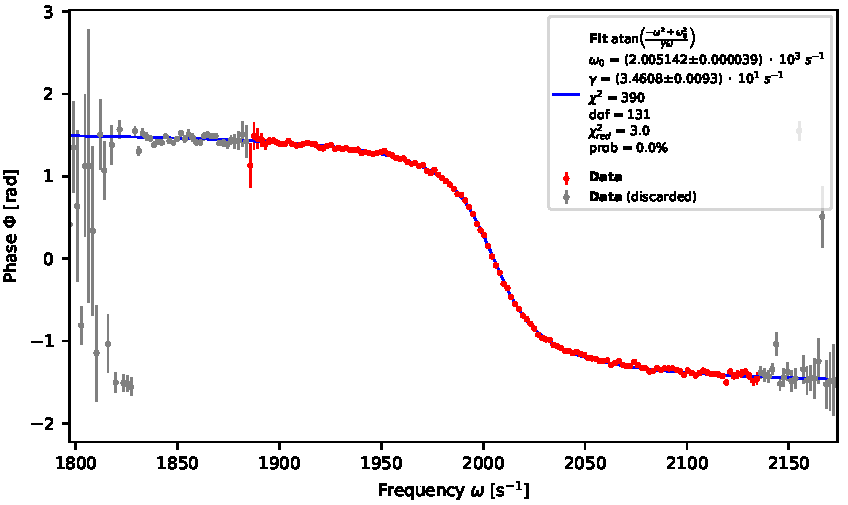
\includegraphics[]{pdf/Phi_0_0}
        \end{adjustbox}
        \begin{adjustbox}{max width=0.45\linewidth, keepaspectratio}
            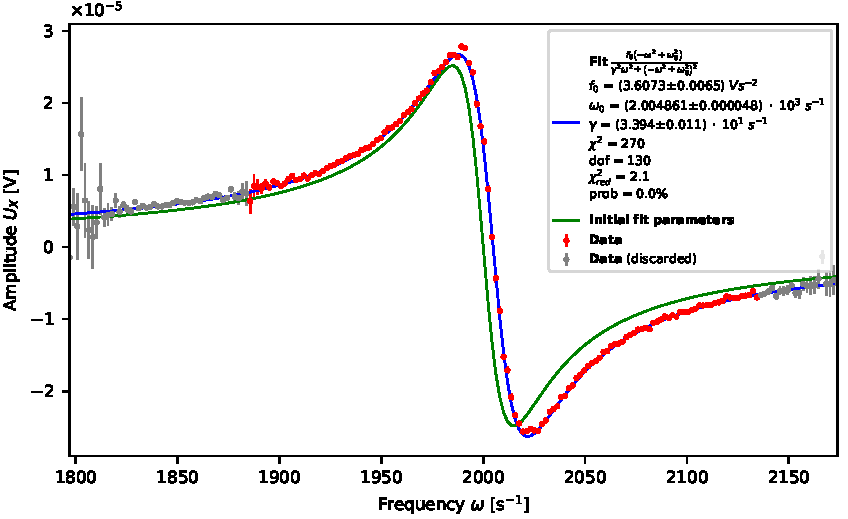
\includegraphics[]{pdf/U_X_0_0}
        \end{adjustbox}
        \begin{adjustbox}{max width=0.45\linewidth, keepaspectratio}
            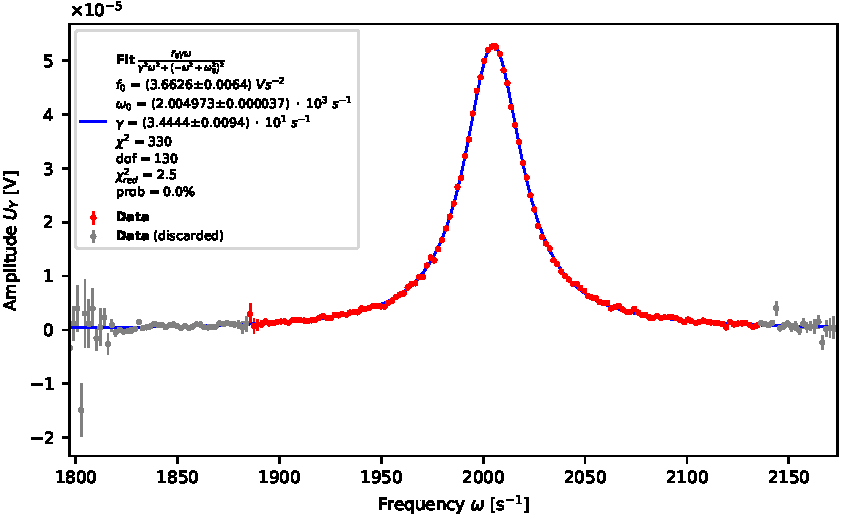
\includegraphics[]{pdf/U_Y_0_0}
        \end{adjustbox}
        \captionof{figure}{Alle vier Auswertungsmöglichkeiten für die erste Mode bei Raumtemperatur. Oben links: Amplitude $A$, oben rechts: Phase $\Phi$, unten links: Signal $U_X$, unten rechts: Signal $U_Y$}
        \label{fig:RaumtempKomplett}
    \end{center}
\endminipage

\minipage{\linewidth}
    \begin{center}
        \captionsetup{type=figure}
        \begin{adjustbox}{max width=0.45\linewidth, keepaspectratio}
            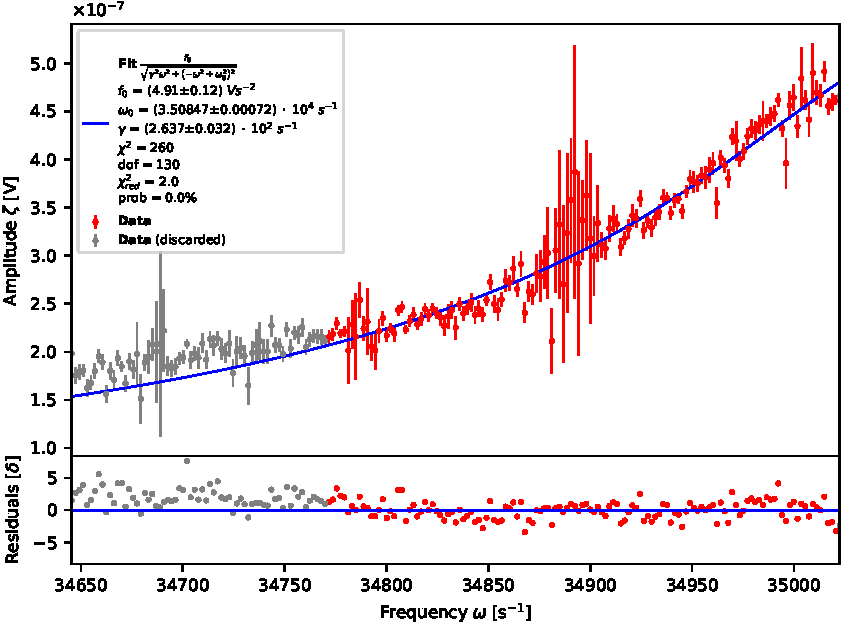
\includegraphics[]{pdf/A_9_2}
        \end{adjustbox}
        \begin{adjustbox}{max width=0.45\linewidth, keepaspectratio}
            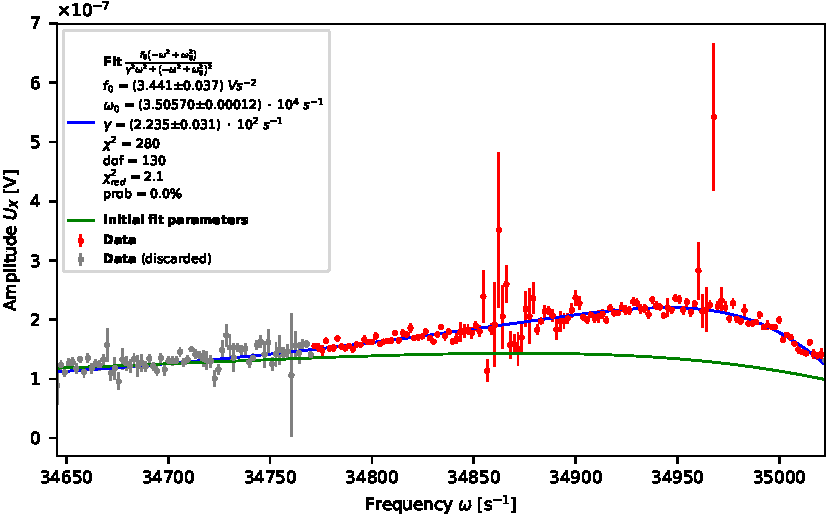
\includegraphics[]{pdf/U_X_10_2}
        \end{adjustbox}
        \captionof{figure}{Der Resonanzbereich wurde für die dritte Mode nicht gut getroffen. Dies wird deutlich bei diesen beiden ausgewählten Plots (links: Amplitude $A$, rechts: Signal $U_X$) höherer Temperaturen - denn hier ist durch die kleinere Resonanzfrequenz der Randbereich des Resonanzbereichs noch erfasst. Wahrscheinlich wurde die Resonanzkurve mit den Artefakten verwechselt, welche im linken Bild gut zu sehen sind.}
        \label{fig:FehlersucheMode3}
    \end{center}
\endminipage

\subsection{Versuchsabschnitt B}

\subsubsection*{Orthogonal-Distance-Regression Fit}

Die im Versuchsabschnitt A bereits berechneten Resonanzfrequenzen $\omega_R$ werden gegen die Temperatur $T$ aufgetragen.
Wir interessieren uns für den anscheinend vorhandenen linearen Zusammenhang.

Der Unterschied in der Auswertung liegt nun darin, dass sowohl $T$, als auch $\omega_R$ mit einer Messunsicherheit belegt ist.
Ein Ordinary-Least-Squares Fit betrachtet jedoch nur die Abweichung der Größe auf der Ordinate.
Stattdessen verwenden wir für diese Messdaten nun also einen Orthogonal-Distance-Regression (ODR) Fit.

Leider kann an dieser Stelle keine Auswertung der Fitgüte stattfinden, da kein einheitlich akzeptiertes Maß darüber existiert, wie es beispielsweise $\chi^2$ für den OLS Fit darstellt.
Auch in der Versuchsanleitung \cite{Anleitung} sind keine weiteren Informationen darüber zu finden.

\subsubsection*{Ergebnisse}

Abbildungen \ref{fig:Temperaturabhaengigkeit0}, \ref{fig:Temperaturabhaengigkeit1} und \ref{fig:Temperaturabhaengigkeit2} zeigen die Ergebnisse der ODR Fits für die drei vermessenen Moden.
Die resultierten Fitparameter sind in den Grafiken eingetragen.

\minipage{\linewidth}
    \begin{center}
        \captionsetup{type=figure}
        \begin{adjustbox}{max width=\linewidth, keepaspectratio}
            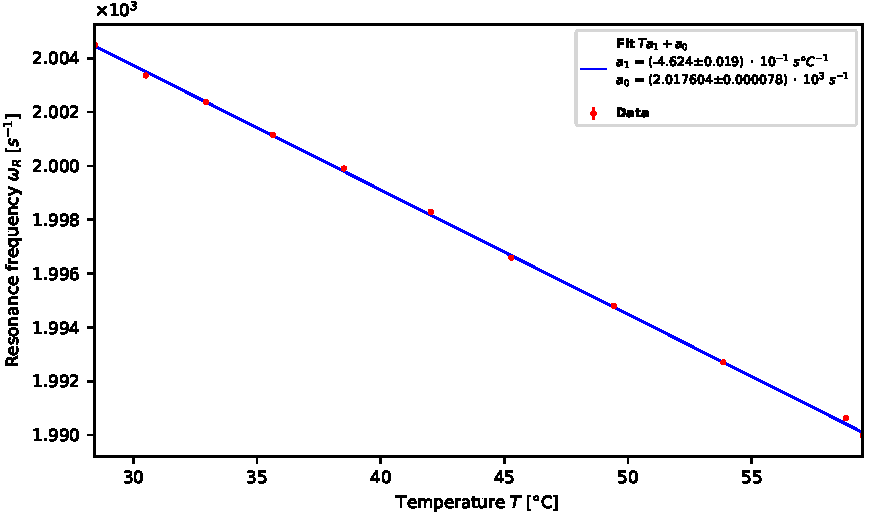
\includegraphics[]{pdf/T_0}
        \end{adjustbox}
        \captionof{figure}{Temperaturabhängigkeit der Resonanzfrequenzen für die erste Mode $\nu_0$}
        \label{fig:Temperaturabhaengigkeit0}
    \end{center}
\endminipage

\minipage{\linewidth}
    \begin{center}
        \captionsetup{type=figure}
        \begin{adjustbox}{max width=\linewidth, keepaspectratio}
            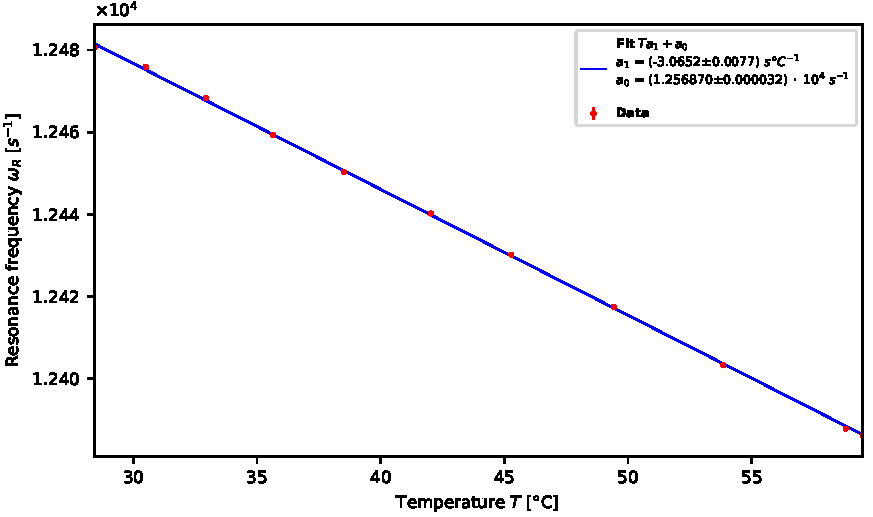
\includegraphics[]{pdf/T_1}
        \end{adjustbox}
        \captionof{figure}{Temperaturabhängigkeit der Resonanzfrequenzen für die zweite Mode $\nu_1$}
        \label{fig:Temperaturabhaengigkeit1}
    \end{center}
\endminipage

\minipage{\linewidth}
    \begin{center}
        \captionsetup{type=figure}
        \begin{adjustbox}{max width=\linewidth, keepaspectratio}
            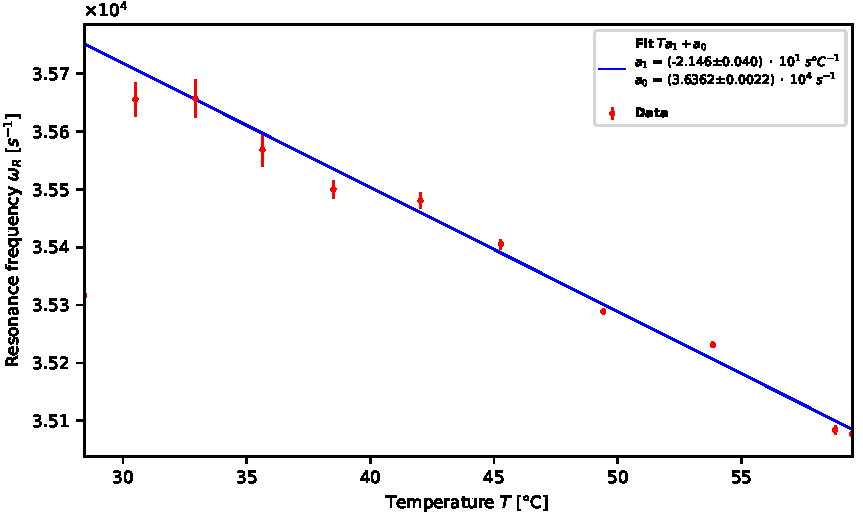
\includegraphics[]{pdf/T_2}
        \end{adjustbox}
        \captionof{figure}{Temperaturabhängigkeit der Resonanzfrequenzen für die dritte Mode $\nu_2$}
        \label{fig:Temperaturabhaengigkeit2}
    \end{center}
\endminipage
